\documentclass[tikz,border=2pt]{standalone}
\usepackage{amsmath,amssymb}
\usepackage{xcolor}
\usetikzlibrary{positioning}
\begin{document}
% Extracted from namuenofull.inc; source column: \footnotesize \cite{NU}$_{\rm p{ 167 }}$ II$^*$-III$^*$-$\alpha$
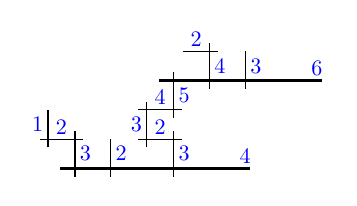
\begin{tikzpicture}[xscale=0.57,yscale=0.62]
\draw[thick,shorten >=2] (4/15,0)--(139/30,0) node[inner sep=2pt,blue,above left,scale=0.8] {4} node[inner sep=2pt,below left,scale=0.8] {};
\draw[shorten <=-3pt, shorten >=-3pt] (3/5,0)--node[inner sep=2pt,scale=0.8,blue,right] {3} (3/5,3/5);
\draw[shorten <=-3pt, shorten >=-3pt] (3/5,3/5)--node[inner sep=2pt,scale=0.8,blue,above] {2} (0,3/5);
\draw[shorten <=-3pt] (0,3/5)--node[inner sep=2pt,scale=0.8,blue,left] {1} (0,6/5);
\draw[shorten <=-3pt] (7/5,0)--node[inner sep=2pt,scale=0.8,blue,right] {2} (7/5,3/5);
\draw[shorten <=-3pt, shorten >=-3pt] (14/5,0)--node[inner sep=2pt,scale=0.8,blue,right] {3} (14/5,3/5);
\draw[shorten <=-3pt, shorten >=-3pt] (14/5,3/5)--node[inner sep=2pt,scale=0.8,blue,above] {2} (11/5,3/5);
\draw[shorten <=-3pt, shorten >=-3pt] (11/5,3/5)--node[inner sep=2pt,scale=0.8,blue,left] {3} (11/5,6/5);
\draw[shorten <=-3pt, shorten >=-3pt] (11/5,6/5)--node[inner sep=2pt,scale=0.8,blue,above] {4} (14/5,6/5);
\draw[shorten <=-3pt, shorten >=-3pt] (14/5,6/5)--node[inner sep=2pt,scale=0.8,blue,right] {5} (14/5,9/5);
\draw[thick,shorten >=2] (37/15,9/5)--(187/30,9/5) node[inner sep=2pt,blue,above left,scale=0.8] {6} node[inner sep=2pt,below left,scale=0.8] {};
\draw[shorten <=-3pt, shorten >=-3pt] (18/5,9/5)--node[inner sep=2pt,scale=0.8,blue,right] {4} (18/5,12/5);
\draw[shorten <=-3pt] (18/5,12/5)--node[inner sep=2pt,scale=0.8,blue,above] {2} (3,12/5);
\draw[shorten <=-3pt] (22/5,9/5)--node[inner sep=2pt,scale=0.8,blue,right] {3} (22/5,12/5);
\end{tikzpicture}
\end{document}
